\subsection{\textit{CKAN}}
  
\textit{\gls{ckan}} is an open-source data management solution whose main objective is to allow the creation, access, and dissemination of knowledge through tools for the use and reuse, publication, search and share of information. Generally, it is implemented by organisations and is used by several national governments to manage their data, but it can also be used by companies, research institutions, or even individuals. Currently, \textit{\gls{ckan}'s} design demonstrates a versatile range of options, and can be used as a catalog, repository, datastore, or as a combination of all three \citep{5}.
  
\subsubsection{Architecture}
  
\textit{\gls{ckan}} follows the classic \textit{Model View Controller (MVC)} pattern. There is a clear distinction between the various layers, where the data representation and client interaction, i.e. the View, are separated from the methods that interact with the databases, i.e. the Model, with the Controller mediating between the two through the changes that the user interacting with the system wants. This architecture is shown in and the Figure \ref{fig:ckan_arch}.
  
\begin{figure}[h!]
    \centering
    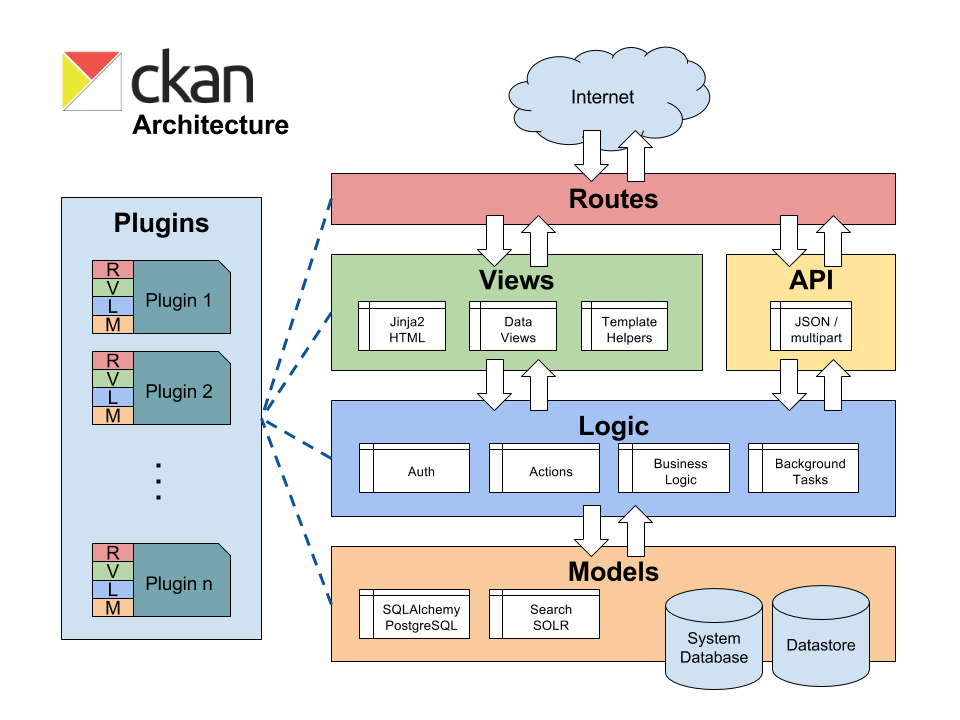
\includegraphics[width=0.9\textwidth]{img/state_of_the_art/architecture_ckan.png}
    \caption{\textit{\gls{ckan}} Code Architecture (http://docs.ckan.org/en/2.9/contributing/architecture.html)}
    \label{fig:ckan_arch}
\end{figure}
    
\textit{\gls{ckan}} is highly customisable and encourages the extension of content to the code base to adapt the system to different needs. The community and the \textit{\gls{ckan}} development team already have a vast list of extensions available.
  
\subsubsection{Installation}
  
The best option for \textit{\gls{ckan}'s} installation, which is currently in version 2.9 (version by which the evaluation of this platform will be guided), depends on the intended use of it. According to the documentation that the system provides, there are three ways to install it: 
  
\begin{itemize}
  \item Install from an operating system package;
  \item Install from source;
  \item Install from \textit{Docker Compose}, a tool for defining and running multi-container \textit{Docker} applications;
\end{itemize}
  
Installing from the package is the fastest and easiest way to get \textit{\gls{ckan}}, as it requires either the 18.04 64-bit or 20.04 64-bit version of Ubuntu. It is still necessary to install \textit{Solr} for the research tools and \textit{PostgreSQL} for the database. Moreover, this system is primarily written in \textit{Python}.
  
When the installation is well completed, two web applications will be running, \textit{\gls{ckan}} itself and the \textit{Datapusher}, a distinct service for automatically importing data to \textit{\gls{ckan}'s} \textit{DataStore} extension.
  
\subsubsection{Datasets, Role management and Authorisation}
  
With \textit{\gls{ckan}}, data is published in units called datasets, which contain two things: information relating to the data, in other words, metadata, and resources that contain the data, which can be stored as relational database entries or separate files (XML files, images or linked data in RDF format, for example).
  
Unlike other cloud services, \textit{\gls{ckan}} does not use a distributed data storage, since multi-user concurrency is not a major requirement in the way this software handles information. Instead, data integrity is generally favoured by data publishers to avoid data conflicts. Hence, \textit{\gls{ckan}}'s team decided to implement a central data store to meet their needs \citep{8}.
  
Typically, each dataset belongs to an organisation and each \textit{\gls{ckan}} instance can have numerous organisations. Considering, for example, the case of a scientific investigation that is being carried out by a research center that is using \textit{\gls{ckan}}, there may be different departments publishing data. In this case, each organisation can define its way of working and specific authorisations, providing tools to manage its data ingestion process. Thus, the platform becomes very versatile and there is no requirement for centralised management.
  
Within each organisation, there can be different levels of access, where admins can add users and specify the level of access for each one.
  
Despite the above, it is also possible to configure \textit{\gls{ckan}} with the objective that the datasets do not belong to any organisation, which opens up the possibility of a wiki-like \textit{DataHub}.
  
\subsubsection{Metadata}
  
By default, \textit{\gls{ckan}} offers the following basic set of metadata:

\begin{itemize}
  \item Title;
  \item ID;
  \item Groups;
  \item Description;
  \item Revision history;
  \item License;
  \item Tags;
  \item Formats;
  \item \gls{api} key.
\end{itemize}
  
It also allows other attributes, such as location data through the geographic feature or customised information relevant to the publisher or dataset. Although the \textit{\gls{ckan}} metadata does not follow any standard schema, the system, through the above-mentioned customisation, grants the inclusion of arbitrary key/value pairs, which can only be represented by strings \citep{1}.
  
\subsubsection{\textit{FileStore} and \textit{DataStore}}

\textit{\gls{ckan}'s} \textit{FileStore} allows users to upload files, which by default are stored locally on the server, so that \textit{\gls{ckan}} has more control over the files and manages access to them. However, some extensions allow the user to save files remotely, such as on \textit{Amazon S3} \citep{5}. Presently, only one storage location can be used.
  
The \textit{DataStore} extension provides a database to store structured data of \textit{\gls{ckan}} resources, and data can be extracted from files and saved in the \textit{DataStore}, whether initially in the \textit{FileStore} or external links. The upload work of both possible resource sources is from \textit{Datapusher}.
  
Therefore, there are two distinct ways of storing \textit{\gls{ckan}} resources. On the one hand, there is the \textit{FileStore} which provides a storage of files where access or filtering to specific parts is not possible. On the other hand, the \textit{DataStore} is like a database where accessing and filtering data elements is possible. For example, a file of the CSV type, in \textit{FileStore} would be stored as a whole and to access its content would be necessary a download, while in \textit{DataStore} it would be possible to access each line of the content of a CSV spreadsheet individually via an \gls{api}, as well as filtering content. Although \textit{\gls{ckan}} does not support data replication, it is possible to say that a partial replication of certain datasets can often occur under the simultaneous use of these two storage components.
  
\subsubsection{Interoperability}
  
Through its \gls{api}s, this system offers tools for developers who want to interact with \textit{\gls{ckan}} sites or their data. In addition to the \textit{\gls{ckan}} Action \gls{api}, an RPC-style \gls{api} that exposes the core functionalities of a \textit{\gls{ckan}} website to any external code, \textit{FileStore}, and \textit{DataStore} have their \gls{api}s. 
  
Despite the interoperability that allows via \gls{api}s, \textit{\gls{ckan}} fails to support, by default, compliance with standard protocols used by the scientific community such as the OAI-PMH. Furthermore, metadata records do not follow any specific schema, despite allowing the use of an extension that exposes and consumes metadata using Resource Description Framework (RDF) documents serialized using Data Catalog Vocabulary (DCAT), which is an RDF vocabulary developed to facilitate the interoperability between data catalogs \citep{4, 5}. Thus, \textit{\gls{ckan}} makes it possible to expose and consume metadata from other data catalogs with standards schemas, but at no point does it include their validation, which in this case is done by the entities that originate the data.
 
This system can be used to create a federated network of data portals that share and manage data with each other. This is achieved through the \textit{\gls{ckan}} harvesting extension, and it is even possible to federate data from \textit{non-\gls{ckan}} catalogs with the aforementioned DCAT extension.
  
\subsubsection{Search, preview and visualization tools}
  
\textit{\gls{ckan}} provides a search interface similar to \textit{Google}, allowing search by word, delimited or not by quotation marks. Users can easily get a list of available datasets and perform searches on them. There are several search options, which can all be performed via \gls{api}:
  
\begin{itemize}
  \item Search on all dataset attributes;
  \item Full-text search;
  \item Fuzzy-matching, option to find terms close to the one entered instead of exact terms;
  \item Faceted search, in other words, searching through specific fields, such as tags.
\end{itemize}
  
This platform can automatically preview some data types and extend an interactive analysis before downloading. The main features of content visualization include graphics, tables, maps (via advanced geospatial features), or images, and it is also possible to create new forms of preview for other types of data through extensions.
  
\subsection{\textit{Magda}}
  
\textit{Magda} is an open-source data catalog system that provides a single space for an organisation's data to be stored, cataloged, searched, and enriched, whether large datasets or small files. This system is designed around the concept of federation and with the flexibility to be used as a catalog of big data in a data lake, an easily searchable repository for small data files, an aggregator of data from multiple external sources, or all in one.
  
\subsubsection{Architecture}
  
One of \textit{Magda's} main characteristics is its architecture, which is presented in a diagram in Figure \ref{fig:magda_arch} and consists of an extensible set of micro services that are distributed as \textit{Docker} containers, in the sense that new services can be added allowing organisations to go beyond the standard system. Any extension to collect data or enrich metadata can be written in any language and added/removed without significant changes to the operation of the core system. The architecture of \textit{Magda} is presented in a diagram in Figure \ref{fig:magda_arch}.
  
The use of \textit{Kubernetes}, for orchestrating \textit{Docker} containers, and \textit{Helm}, which helps manage \textit{Kubernetes} applications, means that the configuration of a customisable \textit{Magda} instance can be stored and tracked as plain text, and instances with identical configuration can be replicated quickly.
  
  
\begin{figure}[!h]
    \centering
    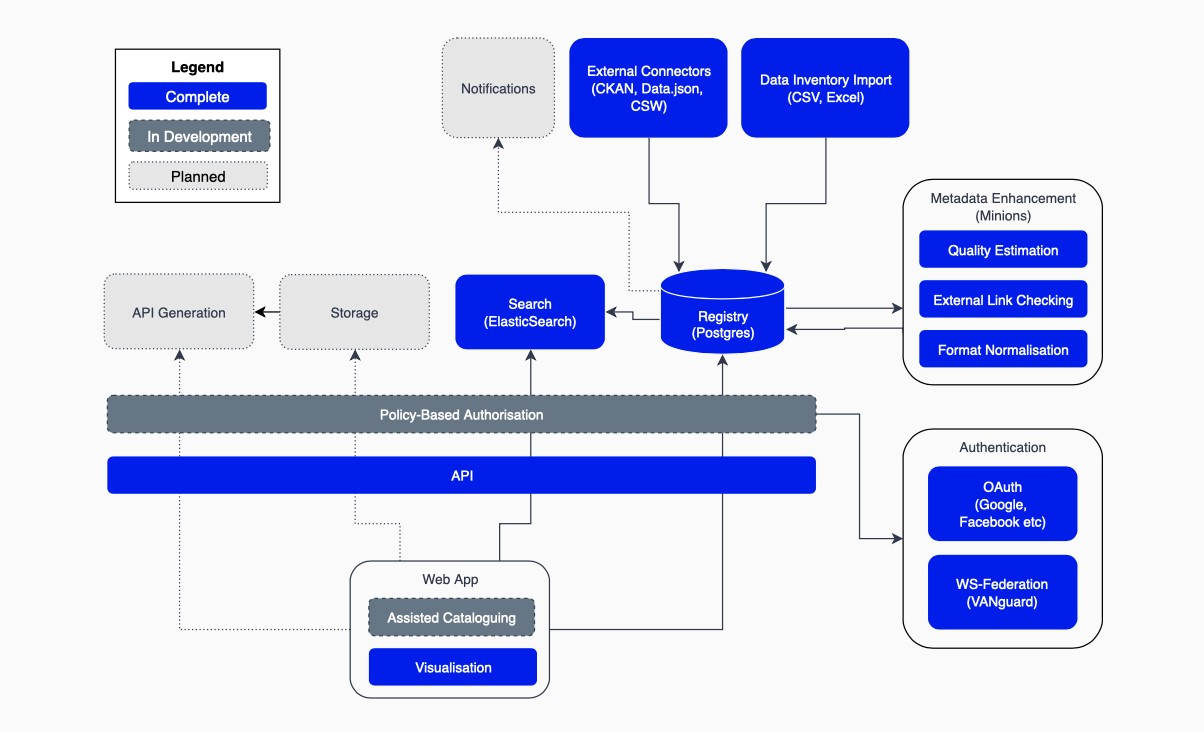
\includegraphics[width=1\textwidth]{img/state_of_the_art/architecture_magda.jpg}
    \caption{\textit{Magda} Architecture (https://magda.io/)}
    \label{fig:magda_arch}
\end{figure}  
  
\newpage  
  
\subsubsection{Installation}
  
\textit{Magda} can be installed in two ways, with the one chosen depending on the priorities of the user or organization:
  
\begin{itemize}
    \item Install from source;
    \item Install from \textit{Terraform}, a tool that provides a workflow for managing cloud services as \textit{Google Cloud}, or via another local or cloud environment.
\end{itemize}

Using \textit{Kubernetes} and \textit{Helm} enables simple installation and minimal system downtime. Configuration via pre-built images, i.e. from the second option in the list above, is simple in a setup as an open data search engine. However, using other features like adding datasets or the admin UI. setup is not so simple and \textit{Kubernetes} skills are usually required.
    
\textit{Magda} is currently under development, with their team looking to make the open source side more robust and adding new features to their implementations, which at the moment are not fully documented or require specific configurations to work.
    
\subsubsection{Authorisation and authentication}
  
At the moment a customisable authorisation system based on Open Policy Agent is being integrated, which will allow:
  
\begin{itemize}
  \item Restricting datasets based on the establishment of access control frameworks (through roles, for example) or policies specified by the organization;
  \item Control user access to content when searching for it;
  \item Federated authorisation.
  \end{itemize}
  
The latter not only allows data to be collected from external sources but also allows to mimic the same authorisations policies.
  
\textit{Magda's} authentication system, which is based on \textit{PassportJS}, an authentication middleware for \textit{NodeJS}, integrates a wide range of providers, such as \textit{Google}, \textit{Facebook}, or even the aforementioned \textit{\gls{ckan}}. In addition, it is also possible to develop authentication plugins to customise this process.
  
\subsubsection{\textit{Registry}}
  
\textit{Magda} works on the basis of a \textit{Registry}, an opinionless datastore built on top of \textit{PostgreSQL}, which stores records as a set of JSON documents called aspects. A dataset is represented as a record with several aspects - basic records containing the name or description, for example, or more complex ones like the quality or license of the data. Similarly, the actual data files or the URLs that link to them are also worked out as records, with their own sets of aspects. 

Aspects can be declared dynamically by other services through a call with name, description, and JSON schema. This allows the user to save extra information by declaring new aspects. Also, since the system is opinionless, it is possible to create new entities in the system that connect to each other.
  
\subsubsection{Metadata and \textit{Minions}}
  
The default metadata format used natively is the aspects system. \textit{Magda} has an unopinionated central metadata store and therefore can provide most metadata schemas but none as standard, i.e. it supports partial standardisation.
  
\textit{Magda} is ready to automatically enhance metadata without ever needing the data to be transmitted to a \textit{Magda} server. The process of adding datasets for those that are cataloged directly is able to derive data from the files directly in the user's internet browser. 
  
A \textit{Minion} is a service that observes new records or changes to existing ones, performs some operation and writes the result back to the \textit{Registry}. There are several aspects that are written by various \textit{Minions}, such as the quality aspect that contains content evaluations from different sources, which are averaged out and used by search. For both internal or external dataset, the \textit{Minions} framework is ready to act.
  
The framework for enhancement can be extended so that the user/organisation can build its enhancement process using any language that can be deployed as a \textit{Docker} container.
  
\subsubsection{Interoperability and \textit{Connectors}}
  
\textit{Magda} is designed with the ability to pull data from external sources into an easily searchable catalog in which all datasets are all one entity that supports all the operations available in the others, regardless of where they come from. However, it does not use any harvesting protocol such as OAI-PMH.
  
For the data collection process there are so-called \textit{Connectors}, \textit{Docker-based} micro services invoked as jobs, which go to external data sources and copy their metadata to the \textit{Registry}. Thus, the metadata can be searched and have other aspects attached to it. 
  
This system can accept metadata from its own cataloging process, and there are Excel or CSV-based data inventories and metadata \gls{api}s such as those from \textit{\gls{ckan}} or from its own REST \gls{api}. Moreover, the data here is combined into a single search index with history tracking and notifications when metadata records change.

\subsubsection{Search, preview and visualisation tools of data}
  
When users search for something they expect the result to be the best and closest to what they want, not just the one that matches the most keywords. This system is ready to return better quality datasets over lower quality ones, understand acronyms and synonyms, and even search for geospatial or time.
  
Datasets and distributions (the actual data files or URLs that link to them) in the \textit{Registry} are fed into an \textit{ElasticSearch} (which is a distributed, scalable and open data search and analysis engine for all kinds of data) cluster, which indexes some key aspects of each and exposes an \gls{api}.

For previewing datasets \textit{Magda} provides tools to verify the usefulness of their representation through graphs, automatic charting of data in tables, and spatial previewing with the open framework called \textit{TerriaJS} for building spatial data federated web platforms.  
  
A User Interface (UI) is provided for these tools, which is served through its own micro service and consumes \gls{api}s. Moreover, there are plans to make this UI extensible in the future.
  
\subsection{\textit{EUDAT}}
  
\textit{\gls{eudat}} is a pan-European Collaborative Data Infrastructure (CDI) initiative (i.e. it involves all or almost all the nations of Europe), which consists of a network of nodes that provide a range of services to integrate, search, share, store, and replicate research data, more some additional services. These nodes are substantially data centers or computing centers that contain a data repository and provide a stack or part of the \textit{\gls{eudat}} services to manage the stored data, and these service providers can be divided into two categories: with specific research theme or generic.
  
\subsubsection{\textit{EUDAT} Services}

Currently, \textit{\gls{eudat}} CDI has the following services:
  
\begin{itemize}
  \item \textit{B2ACCESS}, user authentication and authosisation;
  \item \textit{B2DROP}, store, synchronise and exchange data;
  \item \textit{B2FIND}, metadata harvesting and cataloging;
  \item \textit{B2HANDLE}, persistent identification management;
  \item \textit{B2HOST}, deploy and operate applications and data-oriented services on machines next to the data storage location;
  \item \textit{B2NOTE}, for easily and intuitively create annotations on data;
  \item \textit{B2SAFE}, safe data replication;
  \item \textit{B2SHARE}, store, share and publish data from smaller datasets;
  \item \textit{B2STAGE}, data transfer to high-performance computers.
\end{itemize}
  
  
\begin{figure}[!h]
    \centering
    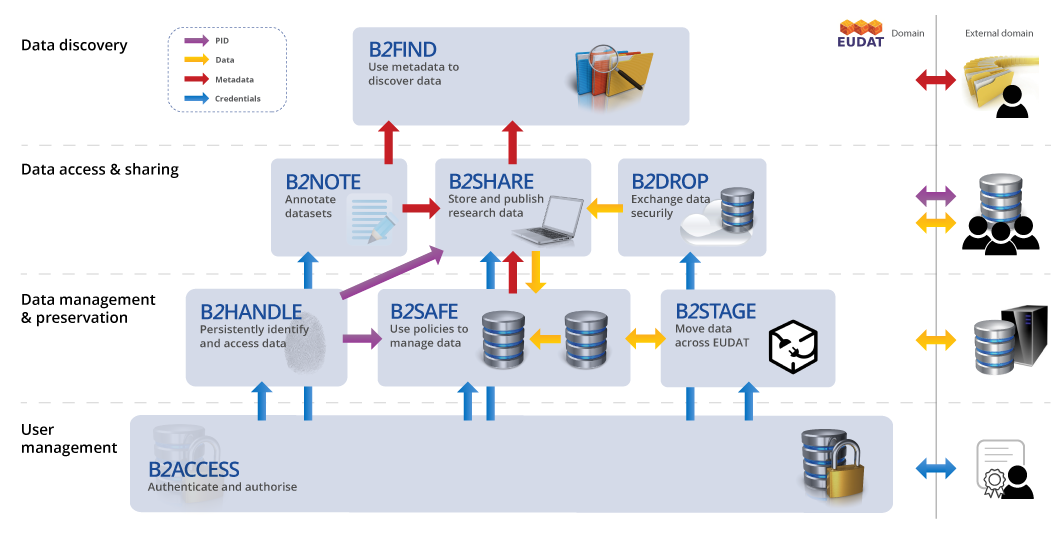
\includegraphics[width=1\textwidth]{img/state_of_the_art/eudat_services.png}
    \caption{\textit{\gls{eudat}} services (https://eudat.eu/services/userdoc/eudat-primer)}
    \label{fig:eudat_services}
\end{figure}
  
\subsubsection{Interaction with \textit{EUDAT} CDI}
  
 The users of the EUDAT common services appear in two layers: researchers as end-users and experts from the scientific communities/organisations \citep{damien}. 
 
 There are two ways in which scientific communities/organisations can integrate with \textit{\gls{eudat}}:

\begin{itemize}
    \item Join: community becomes a data centre or computing centre part of the \textit{\gls{eudat}} network, which is more demanding to develop, but allows close use with all core services. This requires a minimal installation and configuration of the \textit{\gls{eudat}} CDI, and the provision of some resources, such as computing and storage, by the community;
    \item Use: an existing \textit{\gls{eudat}} data centre or computing centre ingests the community data and ensures its storage and also its replication, if desired. Unlike the former, due to the looser interaction, users will have little or no control over the development of core features and their configurations. {\textit{\gls{eudat}}} exposes several UIs (to aggregate them, a {Common Services Layer Interface (CSLI)} is currently under development) and \gls{api}s for using its services.
\end{itemize}

End-users can also use the system in a similar way to community use, however, data replication is not possible for them.
  
\begin{figure}[!htb]
   \begin{minipage}{0.48\textwidth}
     \centering
     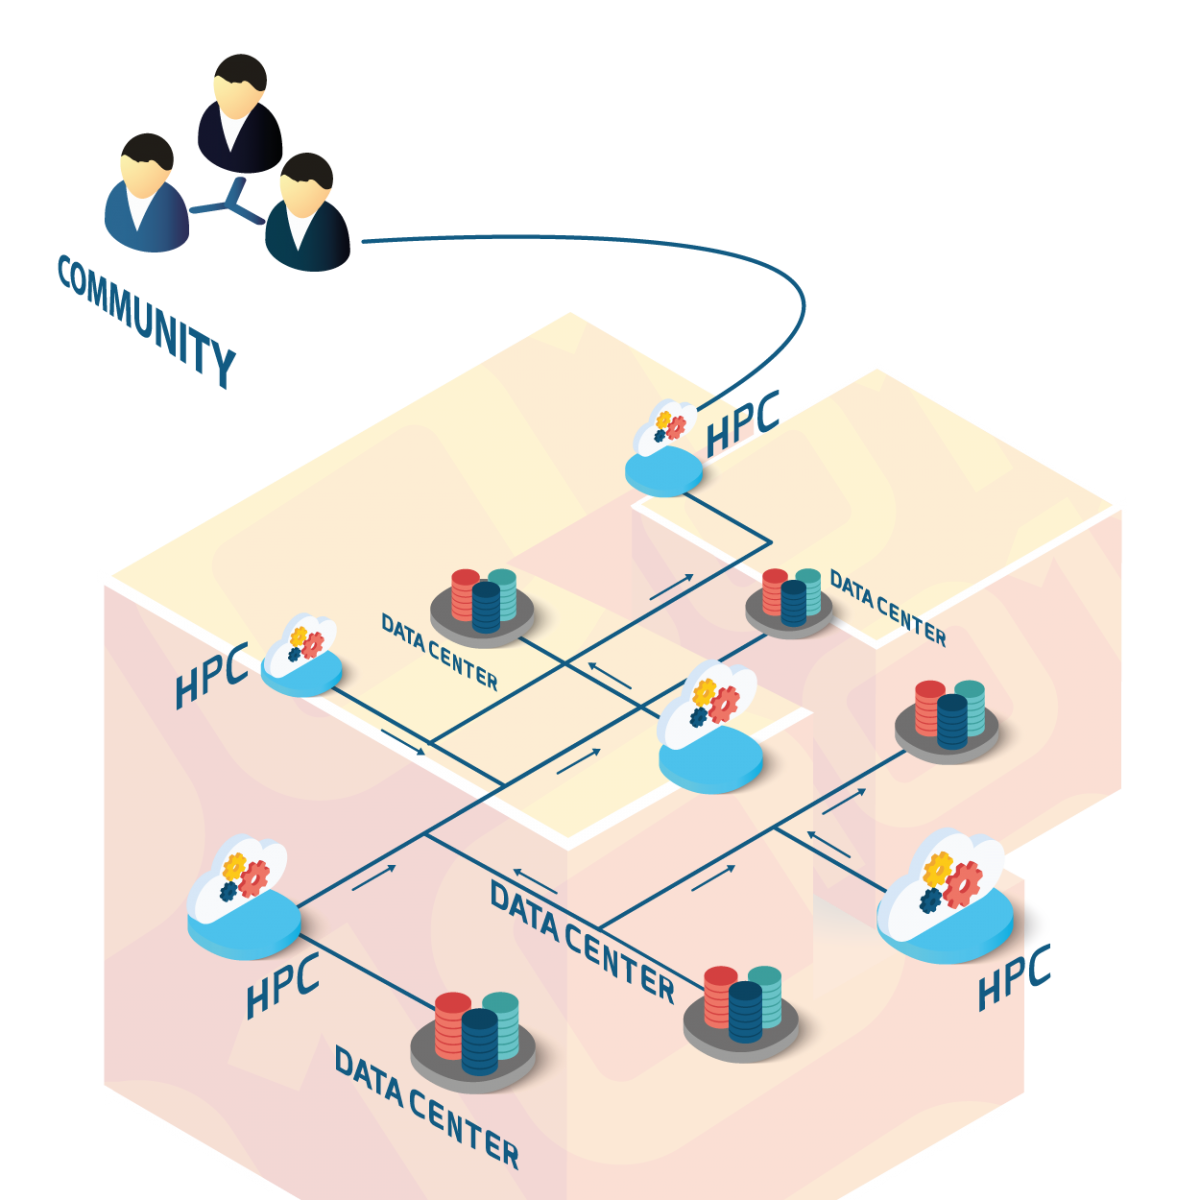
\includegraphics[width=0.85\textwidth]{img/state_of_the_art/use_eudat.png}
     \caption{Using the \textit{\gls{eudat}} services (https://www.eudat.eu/eudat-cdi/using)}\label{Fig:Data1}
   \end{minipage}\hfill
   \begin{minipage}{0.48\textwidth}
     \centering
     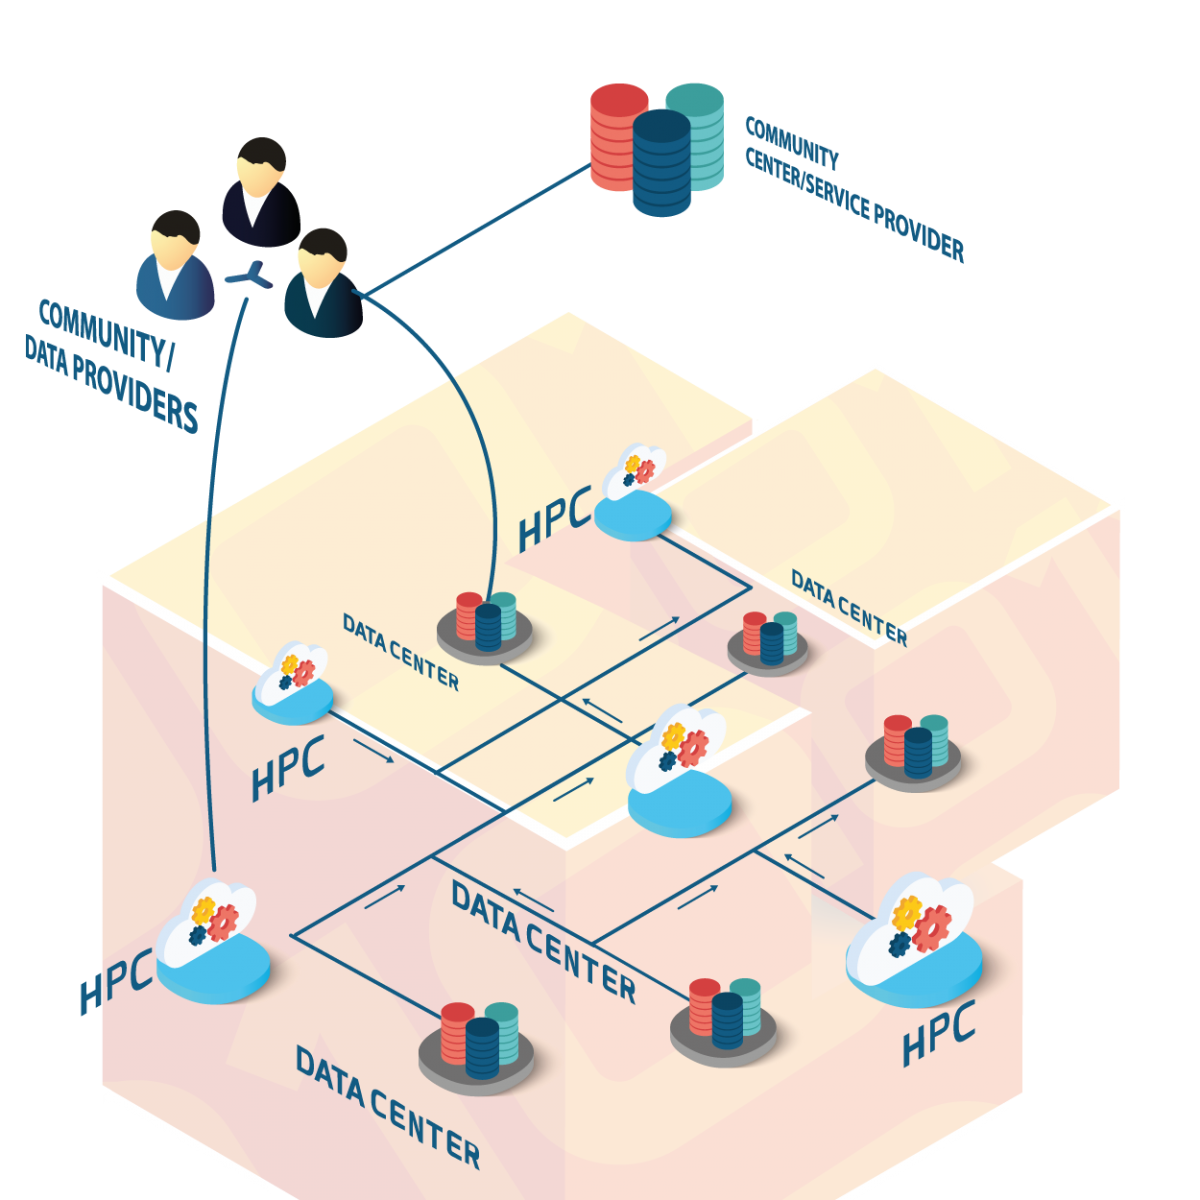
\includegraphics[width=0.85\textwidth]{img/state_of_the_art/join_eudat.png}
     \caption{Joining the \textit{\gls{eudat}} services (https://eudat.eu/eudat-cdi/joining)}\label{Fig:Data2}
   \end{minipage}
\end{figure}
  
In both cases, the community can access \textit{\gls{eudat}'s} primary services, which will be analysed in the next subsection. The following image clearly illustrates the distinction between the two forms of interaction.
  
\begin{figure}[!h]
    \centering
    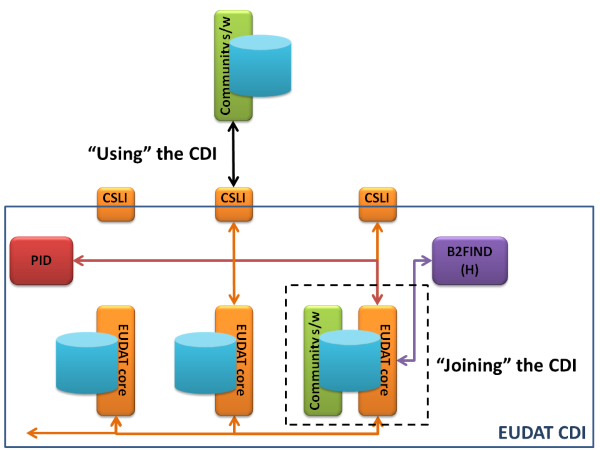
\includegraphics[width=0.6\textwidth]{img/state_of_the_art/use_or_join.png}
    \caption{Interaction with the \textit{\gls{eudat}} CDI (https://eudat.eu/services/userdoc/eudat-primer)}
\end{figure}
  
\newpage
  
\subsubsection{\textit{B2ACCESS}}
  
\label{tab:b2access}  
  
\textit{B2ACCESS} is a federated cross-infrastructure framework for user authentication and authorisation that controls their access to other services and resources.
  
Users can authenticate in several ways: 
  
\begin{itemize}
    \item User's home organisation identity provider;
    \item Social account, like \textit{Google} or \textit{Facebook};
    \item \textit{B2ACCESS} id.
\end{itemize}
  
The \textit{B2ACCESS} process is based on two  aspects - attributes and groups. Attributes are key-value pairs that describe basic user information, such as their name, and keep information for authorisation purposes, such as membership to communities. Groups are used to manipulate and control user's access to other services, with each service having its own set of groups.
  
\subsubsection{\textit{B2DROP}}
  
\textit{B2DROP} is a trustworthy service used by investigators to exchange data and thus keep data synchronised and up-to-date with each other, being based on \textit{NextCloud}.
\textit{B2DROP's} main intention is to be used for volatile data that can be easily change and still subjective for the research and to manage this provides the version of the inserted files but does not maintain persistent identifiers for them. It can be used via a user-friendly web UI or implemented as a drive on the desktop machine via WebDav.
    
\subsubsection{\textit{B2FIND}}
\label{tab:b2find}

Metadata is a key part of data management, as they describe the dataset. Systematically structured and searchable metadata enables efficient discovery of scientific data, and this is how \textit{B2FIND} service works, using a comprehensive joint metadata catalog and a search portal respectively, aided by \textit{\gls{ckan}} functionality and \gls{api}.
  
This service can be used through the discovery portal via the web, an \gls{api}, or an intuitive command-line tool, and encompasses advanced functions like presenting datasets through tables or filtering by location using geospatial features. To search by metadata there are three options, which can even be used together:
  
\begin{itemize}
  \item Free text search, without any restriction;
  \item Faceted search, through specific fields or properties;
  \item By location or time.
\end{itemize}
  
\textit{B2FIND} aggregates diverse metadata information from heterogeneous sources within \textit{\gls{eudat}}. Regarding protocols for metadata, the standard is OAI-PMH, but other formats are also possible. 
  
The metadata schema is based on \textit{DataCite} schema but is compatible with others, such as DublinCore. Currently it includes 26 elements with different levels of obligation: mandatory if applicable; recommended; optional. Some of these elements incorporate important particularities related to the content, such as the use of persistent identifiers of resources (the DOI being specifically intended to make citation available), or information about its licensing and consequent permission status for use by other researchers. 
  
The use of a metadata schema and collection protocols such as these add a validation component in the process of improving metadata quality, a process in which \textit{B2FIND} is embedded.
  
\subsubsection{\textit{B2HANDLE}}
  
\textit{B2HANDLE} is a distributed service that handles the management of Persistent Identifiers (PIDs) based on the \textit{Handle} system, a trusted and scalable software infrastructure used by data curators focused on identifier registration services to create and control identifiers of their resources. The \textit{Handle} system for referencing PIDs uses a string as a prefix and a suffix separated by a "/". 
  
Communities that join \textit{\gls{eudat}} and want to provide this service can do so in two ways: either the data center itself runs \textit{Handle} or they pass their prefix to a \textit{\gls{eudat}} partner to manage the control. Thus, \textit{B2HANDLE} improves interoperability and makes operations of other services easier.
  
Other \textit{\gls{eudat}} services use this to ensure access to data from a long-term perspective, as well as its maintenance. Specifically, \textit{B2FIND} and \textit{B2STAGE} use \textit{B2HANDLE} to query objects and \textit{B2SHARE} and \textit{B2SAFE} to create and manage the PIDs of the data objects they store.
    
\subsubsection{\textit{B2HOST}}
  
Some members of \textit{\gls{eudat}} service providers -- Tieteen Tietotekniikan Keskus Oy (CSC) , Jülich Research Centre (JUELICH), Max Planck Gesellschaft (RZG) and SURFsara Bv (SURFsara) -- offer computing resources from their data centres through a service hosting framework called \textit{B2HOST}. These resources provide communities the ability to deploy and work their data-driven applications and services on machines close to the location of the data storage, since extra computing power may be required when the volume of data is too large to be transferred or there may be licensing restrictions that do not allow data to be copied to third parties. 
    
\subsubsection{\textit{B2NOTE}}
  
\textit{B2NOTE} is \textit{\gls{eudat}'s} latest service and offers creation and control of annotations on online resources, which can be comments and/or pointers that provide extra information about a resource.
Three types of annotations are possible: a semantic tag; a free-text keyword for when a specific semantic term is not found; a free-text comment. These are stored and can later be searched, and the results can be viewed via UI and refined before being exported or as JSON-LD (JSON for linked data).

At the moment this service is still being finalised and is not integrated into the other services.

\subsubsection{\textit{B2SAFE}}
  
\textit{B2SAFE} is \textit{\gls{eudat}}'s service that provides long-term data preservation through replication to multiple backup sites to ensure data redundancy.
  
This service is implemented as an \textit{iRODS (Rule-Oriented Data System)} -- data management software used in research worldwide module -- with \textit{Handle} REST \gls{api} or the EPIC \gls{api} (system with the same purpose as \textit{Handle}) that serves for the creation and management of PIDs and also uses the \textit{iRODS} middleware to replicate datasets from a datacenter as a source. Communities can ask another \textit{\gls{eudat}} site to host this service and responsibility. 
  
Lastly, each data object, original or replica, is assigned with a PID, which even contains information connecting it to its parents if it is a replica, or to a list of direct children if it is the original.
    
\subsubsection{\textit{B2SHARE}}
  
\textit{B2SHARE} web-based service is a solution that ensures the long-term persistence of locally stored data and enables researchers to publish, store and share small or medium-sized datasets. This service uses other \textit{\gls{eudat}} services for data reliability and retention, while storage is managed by trusted nationally supported repositories.
   
Any user, registered or not, can search for data on the \textit{B2SHARE} homepage. However, it is also possible to deploy \textit{B2SHARE}, requiring a web server or cloud infrastructure as a well as a way to store the published data, and this same deployment can be done through \textit{Docker} containers. In addition, this service is the only one that is open-source.
  
This service has the particularity of being integrated with \textit{B2DROP}, which allows data to be added from it to \textit{B2SHARE}. Besides, the existing data in \textit{B2SHARE} can be searched through the search portal provided by \textit{B2FIND}, which harvests the metadata present in this service.
    
\subsubsection{\textit{B2STAGE}}
  
The \textit{B2STAGE} service offers data staging, in other words, the transfer of data between nodes for processing. There are two protocols for this: GridFTP for large datasets and HTTP for small to medium files.
  
Big Data computing manages a high volume of data and when there are several supercomputers involved is necessary to take data transfer even more seriously. The implementation of this service is currently limited to files managed by \textit{B2SAFE}, handling the dynamic replication of data to the \gls{hpc}s. It also provides a \textit{B2STAGE} HTTP \gls{api} for dynamic access to data for integration into specific community applications.
  
\subsection{Evaluation}
  
The evaluation of the three systems analysed in the previous section is done based on the criteria also listed in the previous section, and is provided in Table \ref{tab:arch_comparison} to \ref{tab:usa_sec_comparison}. It should be noted that for the last table, the first field regarding popularity instead of being evaluated with a (\checkmark) or (\xmark)  is evaluated in order of popularity. 
  
\textit{\gls{ckan}} is already sucessful in several cases of government data platforms such as the US, corporate data platforms such as Lego, and is also used by the European Data Portal's, whose commitment to open research data and learning is paramount, with over 35 countries involved. \textit{\gls{eudat}}, meanwhile, has more than 25 member, all data centers and research organizations, such as CERN (European Organization for Nuclear Research). Finally, \textit{Magda} has as its only case of success its initial goal, which was to develop a federal government data portal for the government of Australia.
  
\begin{table}[h!]
    \begin{threeparttable}[b]
    \centering
    \caption{\label{tab:arch_comparison}Architecture comparison}
    \begin{tabular}{>{\centering\arraybackslash}p{1.75cm}>{\centering\arraybackslash}>{\centering\arraybackslash}p{3.5cm}>{\centering\arraybackslash}p{1.5cm}>{\centering\arraybackslash}p{2.5cm}>{\centering\arraybackslash}p{1.8cm}>{\centering\arraybackslash}p{3cm}}
        \hline
        \textbf{Platform} & \textbf{Installation and deployment} & \textbf{Open Source} & \textbf{Storage Replication} & \textbf{Storage Location} & \textbf{Customisation}   \\ 
        \hline
        \textit{\gls{ckan}}              & Installation package or service &       \checkmark                 & \xmark                           & Local or remote\tnote{1}          & \checkmark                            \\
        \textit{Magda}             &  From source or service                     & \checkmark                             &  \xmark                         &  Local or remote                       &  \checkmark             \\
        \textit{\gls{eudat}}             &  Service                     & \xmark\tnote{2}                             &  \checkmark                         & Remote                    & \xmark    \\
        \hline
    \end{tabular}
    \begin{tablenotes}
       \item [1] Remote only available through extensions
       \item [2] Only one service supports this feature
     \end{tablenotes}
    \end{threeparttable}
\end{table}
 
  
\begin{table}[h!]
    \begin{threeparttable}[b]
    \centering
    \caption{\label{tab:int_metadata_comparison} Interoperability \& metadata comparison}
    \begin{tabular}{>{\centering\arraybackslash}p{1.6cm}>{\centering\arraybackslash}p{1cm}>{\centering\arraybackslash}p{2.25cm}>{\centering\arraybackslash}p{1.75cm}>{\centering\arraybackslash}p{2cm}>{\centering\arraybackslash}p{2cm}>{\centering\arraybackslash}p{1.25cm}>{\centering\arraybackslash}p{1.75cm}}
        \hline
        \textbf{Platform } & \textbf{\gls{api}s} & \textbf{Harvesting protocols} & \textbf{Standard schemas}  & \textbf{Validation} & \textbf{Federation} & \textbf{DOI} & \textbf{Licensing}  \\ 
        \hline
        \textit{\gls{ckan}}               & \checkmark           & \checkmark\tnote{1}  &  \checkmark\tnote{1}                       & \xmark                      & \checkmark\tnote{1}         & \checkmark\tnote{1} & \checkmark                       \\
        \textit{Magda}              &  \checkmark              & \xmark               & \xmark\tnote{2}               &  \xmark & \checkmark  &  \xmark  & \checkmark                                      \\
        \textit{\gls{eudat}}              &  \checkmark             & \checkmark             &  \checkmark               & \checkmark               & \checkmark &  \checkmark     & \checkmark                                \\
        \hline
    \end{tabular}
    \begin{tablenotes}
       \item [1] Only available through extensions
       \item [2] Only partially
     \end{tablenotes}
    \end{threeparttable}
\end{table}

\newpage


\begin{table}[h!]
    \centering
    \caption{\label{tab:usa_sec_comparison}Usability \& security comparison}
    \begin{tabular}{>{\centering\arraybackslash}p{1.75cm}>{\centering\arraybackslash}p{2cm}>{\centering\arraybackslash}p{2cm}>{\centering\arraybackslash}p{2cm}>{\centering\arraybackslash}p{4cm}>{\centering\arraybackslash}p{2cm}}
        \hline
        \textbf{Platform}  & \textbf{Popularity}  & \textbf{Advanced search} & \textbf{Geospatial tools} & \textbf{Authorised authentication} & \textbf{Curation workflow}   \\ 
        \hline
        \textit{\gls{ckan}}               & 1º                              & \checkmark                  & \checkmark                     & \checkmark  & \xmark                   \\
        \textit{Magda}              & 3º                      &  \checkmark                   &   \checkmark                  &         \xmark      & \xmark                                \\
        \textit{\gls{eudat}}              & 2º                     &   \checkmark                  & \checkmark                    &   \checkmark & \checkmark                      \\
        \hline
    \end{tabular}
\end{table}
  
After the analysis and evaluation, \textit{\gls{ckan}} is the one that stands out the most. Although it has more cases of proven success in the use made by government institutions for processing their data, the fact that it is an open-source system, has a wide range of features, powerful \gls{api}s, and the possibility of customisation and extensions of functionalities make it possible to use it as a \gls{sdms} \citep{1}. In addition, it gives the option (even incentive) to organisations to have full control over the storage of their data, which can be a key decision for many scientific institutions.

An interesting fact is also the use of \textit{\gls{ckan}} by the other two systems addressed, \textit{\gls{eudat}} in the use of the search portal and \textit{Magda} in metadata aggregation, which demonstrates its value as a solution for data management.
  
There would have been other criteria that could have been taken into account, but this dissertation has focused on those we considered to be the most important in the current choice of a system that is as efficient for large institutions as for smaller ones, whose community support in the development of the platform is somewhat advantageous. 

Apart from the evaluated systems, i.e. \textit{\gls{ckan}}, \textit{Magda} and \textit{\gls{eudat}}, we enunciate other solutions that would be interesting to analyse, such as:
  
\begin{itemize}
    \item \textit{DSpace}, which focuses on creating open source repositories for scholarly and published digital content and shows a few similarities to what \textit{\gls{ckan}} offers. This software package was developed by MIT and HP Labs and has notorious examples of its use such as Apollo (Cambridge University repository) or the Open Knowledge Repository (World Bank repository);
    \item \textit{Invenio}, an open source repository software offering tools for managing digital content in institutional repositories and research data management systems (RDMSs). It was initially developed by CERN, but is also used by other institutions such as the SLAC National Accelerator Laboratory, a U.S. Department of Energy laboratory operated by Stanford University;
    \item \textit{Dataverse}, an open source web application similar to \textit{\gls{ckan}}, but with a greater focus on research data. This project was developed by an institute at Harvard University and of particular note is its use as national solutions for university repositories, proven, for example, in the Netherlands and currently being developed in Norway.
\end{itemize}

Finally, before we proceed to the development of a \textit{\gls{ckan}} based system and its consequent qualitative and quantitative evaluation, we will qualitatively evaluate a \textit{\gls{eudat}} system adapted to our case study. As we have seen in this chapter, the potential of \textit{\gls{eudat}} in the future, if made available for development, could be even more powerful than the \textit{\gls{ckan}} system, so it is in our interest to understand how we could set it up.

\subsubsection{EUDAT}

We now address how our system, which will be developed through \textit{\gls{ckan}}, could have been developed in \textit{\gls{eudat}}. It would also be interesting for us to make a quantitative evaluation, but after contacting the \textit{\gls{eudat}} team, they were inflexible in providing unlimited access to their services for local development purposes, since their integration policy is somewhat rigid. Despite this, they have some workloads for some of their services to be developed locally, but mostly without any support or with the need to get in touch with communities of other software.

Through the experience we have gained through the use of \textit{\gls{eudat}} services in production mode, and through some local reproductions of some of its services, we have been able to understand how we can take advantage of the system considering our case study. We therefore examined which services would be interesting to implement:

\begin{enumerate}
    \item \textit{B2ACCESS}: in order to take advantage of most \textit{\gls{eudat}} services, it is necessary to register on the platform responsible for simple and secure authentication and authorisation. There are several possibilities for authentication, however, we can take advantage of \gls{inesctec}'s existence as an organisation already inserted in the system and authenticate ourselves by providing the identity of the user's organisation of origin. Therefore, it is already possible to access the remaining services without any restriction;
    \item \textit{B2DROP}: after accessing \textit{\gls{eudat}}, the first service to use would be \textit{B2DROP}, which is used to store and exchange data between colleagues in the research team. In this case, the data to be stored in this service would be \gls{gnss} and \gls{nmea}, as these formats do not allow their usability and would need to be processed. This platform allows the insertion of files with a maximum of 2 GB and each user has a maximum quota of 20 GB, which we believe would fit the amount of information resulting from the \gls{sail} Project;
    \item \textit{B2SHARE}: Once we have considered the \textit{B2DROP}, it makes sense to understand where we could store and publish the already processed data, this is where \textit{B2SHARE} comes in, which serves that purpose. In addition, it guarantees the long-term preservation of that same data (through a PID associated to the dataset), which is ideal for those we already consider as final such as the CSV files of the measurements of atmospheric conditions. Thus, while \textit{B2DROP} does not allow metadata, \textit{B2SHARE} already does, and so we could enjoy the use of time and location as some of the fields. When it comes to values, \textit{B2SHARE} allows to upload files up to 10GB and records up to 20GB;
    \item \textit{B2HANDLE}: the acquisition and management of the PIDs made by this service can be entrusted to the \textit{B2HANDLE} team, it is only necessary to acquire a production prefix, which is requested to the team through a form;
    \item \textit{B2FIND}: Although \textit{B2SHARE} shares data and we can search through its platform, this is limited, since its purpose is not that. However, this component is important in the research project of \gls{sail} and, then, the use of \textit{B2FIND} arises, which harvests metadata from different sources, including \textit{B2SHARE}, and includes a data portal (based on \textit{\gls{ckan}}) that allows searching them. To publish the metadata in \textit{B2FIND} it is not enough to have them in \textit{B2SHARE}, we must take into account the protocol we offer to provide the metadata, which is preferably the OAI-PMH protocol, and their schema. Regarding the first point, the OAI-PMH protocol has already been taken into account when preparing the \gls{sail} data management plan and, regarding the second point, one of the schemas considered in that same plan is Dublin Core, which is one of the formats recognised by \textit{\gls{eudat}}. As such, no change would be necessary and it would be sufficient to have the metadata present in \textit{B2SHARE}. 
\end{enumerate}

After evaluating these services, we summarize the reasons why we would not consider the rest in the integration of a system adapted to \textit{\gls{eudat}}:

\begin{enumerate}
    \item \textit{B2NOTE}: the possibility to have annotations to resources is something interesting and that we could contemplate in the system, but it is not yet integrated in \textit{\gls{eudat}} services and is therefore unavailable;
    \item \textit{B2SAFE}: this service emerges as a solution for communities without archiving facilities or without considerable computing resources, which basically need to replicate their data in different data stores. This is not the case in our situation, because an infrastructure like \gls{macc} would have the resources to take control of the system;
    \item \textit{B2STAGE}: required to transfer data in an \gls{hpc} environment, between different data stores, which would be useful when using the \textit{B2SAFE} service.
\end{enumerate}
  